\documentclass[a4j,12pt,landscape]{jarticle}
\topmargin=3mm \headheight=0mm \headsep=0mm
\textheight=170mm 
\textwidth=225mm
\evensidemargin=0mm \oddsidemargin=0mm
\footskip=0mm
\parindent=0cm

%\usepackage[all]{xy}
\usepackage{amssymb}
\usepackage{amscd}
\usepackage{color}
\usepackage{amsmath}
\usepackage[dvipdfm]{graphics}
\usepackage{graphicx}
\usepackage{amsthm}

\pagestyle{empty}

\def\modulo{{\rm mod}}
\def\F2{{\mathbb F}_2}
\def\wt{{\rm wt}}
\def\wo{{\rm wt}_o}
\def\wf{{\rm wt}_f}
\def\UL{{\rm ul}}
\def\bx{{{\mathbf x}}}
\def\by{{{\mathbf y}}}
\def\bw{{{\mathbf w}}}
\def\bu{{{\mathbf u}}}
%\newcommand{\lshift}[1]{{\large $\mbox{#1}\atop<<$}}
%\newcommand{\rshift}[1]{{\large $\mbox{#1}\atop >>$}}

\title{}
\author{}
\date{\today}

\begin{document}
\Huge

%\vspace*{2cm}
\begin{center}
{\bf Simple and Fast MT:\\
  A Two times faster new variant of \\
  Mersenne Twister}
\vspace{1cm}

Mutsuo Saito (Hiroshima Univ.) \\
and \\
Makoto Matsumoto (Hiroshima Univ.).\\
August 12-18 MCQMC 2006
\end{center}
\vspace{\fill}
\parbox{19cm}{\Large
This study is granted in part by
JSPS Grant-In-Aid \#16204002, \#18654021
and JSPS Core-to-Core Program No.18005.
}
\parbox{2cm}{\vskip 1cm \includegraphics*[width=4cm,height=4cm]{logo.jpg}}
%\vskip 1cm 
%\includegraphics*{logo.jpg}

\newpage
We propose \textcolor{blue}{SFMT} pseudorandom numbergenerator.

\begin{itemize}
\item 
SFMT is an $\F2$-linear generator,
whose recursion fits to 

Single Instruction Multiple Data (SIMD)
instructions 

($\approx$ 128-bit operations).

\item
SFMT is \textcolor{blue}{twice faster} than the Mersenne Twister

coded in SIMD.

\item
SFMT is \textcolor{blue}{4 times faster} than the original Mersenne Twister.

\end{itemize}
% \vskip 5mm
% An algorithm to compute the dimension 
% of equidistribution 

% of a 32-bit integer sequence
% generated by 128-bitwise operations

% (by weighted norm).

% $\Rightarrow$ Appendix A

% \newpage
% \noindent
% {\bf 1. Pseudo Random Number Genarator}\\

% In this talk, PRNG is a (finite state) automaton consisting of:
% \begin{itemize}
% \item State set $S$. 
% \item Transition function $f:S \to S$.
% \item Initial state $s_0 \in S$.
% \item (No imput considered.)
% \end{itemize}
% Change the state as follows:
% $$
% s_0 \mapsto s_1:= f(s_0) \mapsto s_2:=f(s_1) \mapsto \cdots.
% $$

% \newpage
% Let $O$ be the set of output symbols.

% (In this talk, we assume $O$=32-bit integers.)

% \vskip 1cm
% At each state $s$, 
% the output is determined by 
% \begin{itemize}
% \item an output function $o:S \to O$.
% \end{itemize}
% The output sequence becomes
% $$
% o(s_0),o(s_1),o(s_2),\ldots.
% $$
% We use this as a pseudo-random sequence.
% \newpage
% \begin{center}
% \includegraphics[width=0.7\linewidth]{figure01.eps}
% \\
% Figure 1: Automaton.
% \end{center}

 
% \newpage
% \noindent
% {\bf 2. Feedbacked Shift Regiter}\\
% In the above automaton, 
% its period is bounded  \\
% by the number of the states $\#(S)$.

% \vskip 5mm
% We want large $S$ (like 20000 bits), \\
% which admits fast computation of $f$ \\
% in a software implementation.

% \vskip 5mm
% Feedbacked Shift Register (FSR) permits $f$ \\
% with $O(1)$-time complexity.

% \newpage
% Feedbacked Shift Register.
% \begin{itemize}
% \item
% $S=$an array of words(=32-bit integers) of length $N$:
% $$
% S = \{(\bw_0,\ldots,\bw_{N-1})| \bw_i \mbox{: 32-bit integer}\}.
% $$
% \item
% $f:(\bw_0,\ldots,\bw_{N-1}) \mapsto (\bw_1,\ldots,\bw_{N-1}, \by)$,

% where $\by$ is given by a function $g$
% $$\by:=g(\bw_0,\ldots,\bw_{N-1}).$$
% \end{itemize}

% Round robin reduces the computation of $f$ to that of $g$. 

% For high speed generation, $g$ looks at only a few words \\
% in the state array.
% \newpage

% \begin{center}
% \includegraphics[width=0.7\linewidth]{figure02.eps}
% \\
% Figure 2: Feedbacked Shift Register.
% \\
% \end{center}
% \newpage
% \noindent
% {\bf 3 Linear Generator}

% We identify: 
% \begin{itemize}
% \item 
% a bit $\{0,1\}$ with the two element field $\F2$, and
% \item 
% 32-bit integer with horizontal vector $\F2^{32}$.
% %\item 
% %128-bit integer with horizontal vector $\F2^{128}$.
% \item 
% Regard $S$ as an $\F2$-vector space.
% \end{itemize}
% An automaton is said to be {\em $\F2$-linear} if 
% the transition function $f$ and 
% the output function $o$ are both $\F2$-linear. \\
% ~~~We consider only this kind of automata, with 
% justification:
% \begin{itemize}
% \item the period is computable
% \item some kinds of assurance on the distribution \\
% (such as the dimension of equidistribution) can be given
% \item can be converted to a non-linear sequence 
% by using a non-linear transform. 
% \end{itemize}

% \newpage
% \noindent
% {\bf 4. Examples of Linear FSR}

% {\bf GFSR} ('73, Lewis-Payne)
% $$
% g(\bw_0,\ldots,\bw_{N-1}) = g(\bw_0, \bw_M) = \bw_0 + \bw_M.
% $$
% The function $g$ reads only two words, so this is called \\
% a two-tap FSR.

% Period is $2^N-1$.

% \newpage
% {\bf Twisted GFSR} ('92, '94, Matsumoto-Kurita)
% $$
% g(\bw_0,\ldots,\bw_{N-1}) = g(\bw_0, \bw_M) = \bw_0A + \bw_M,
% $$
% where $A$ is a ($32\times 32$)-matrix over $\F2$, defined by
% $$
% \bx A = 
% \left\{\begin{array}{ll}
%   \mbox{shiftright}({\bf x}) & (\mbox{if LSB of $\bx$ is 0}) \\
%   \mbox{shiftright}({\bf x})\oplus{\bf a} & 
%   (\mbox{if LSB of $\bx$ is 1}),
% \end{array}\right.
% $$
% where ${\bf a}$ is a constant vector.
% Period is $2^{32N}-1$. 
% \begin{center}
% \includegraphics[width=0.6\linewidth]{figure03.eps}
% \\
% Figure 3: Twisted GFSR
% \end{center}
\newpage
{\bf 1. Mersenne Twister} (MT, '98 Matsumoto-Nishimura)

Let $\F2$ be the two element field.

Identify $32$-bit integers with 
horisontal vectors in $\F2^{32}$.

Consider a recursion of order $N$ over $\F2^{32}$:
$$
\bx_{i+N}:=g(\bx_i, \bx_{i+1}, \ldots, \bx_{i+N-1}).
$$


MT uses an $\F2$-linear recursion
$$
g(\bw_0,\ldots,\bw_{N-1}) = g(\bw_0, \bw_1, \bw_M) = (\bw_0|\bw_1)A + \bw_M,
$$
where $(\bw_0|\bw_1)$ denotes
the concatenation 

of $32-r$ MSBs of $\bw_0$ and $r$ LSBs of $\bw_1$,

and $A$ is a $(32\times 32)$-matrix 
for which $\bw A$ is computable 

by a few bit-operations.

\newpage
Its period is $2^{32N-r}-1$, chosen to be a Mersenne prime.

\vskip 5mm

Choose a constant $32\times 32$ matrix $T$, 
and output
$$
\bw_0T , \bw_1T, \bw_2T, \ldots
$$
to improve the distribution of higher bits (called tempering).
\newpage
\begin{center}
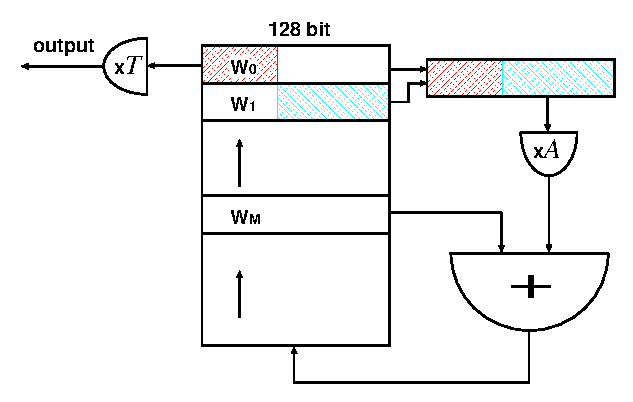
\includegraphics[width=0.9\linewidth]{mt-a.eps}
\\
Figure 1: Mersenne Twister
\end{center}
\newpage
\noindent
{\bf 2. New features of modern CPUs for PCs.}

Modern CPUs for Personal Computers have new features, 
which was not available for standard CPUs 
when MT was designed.
\begin{description}
\item[Multiplication.]
Integer Multiplication is now quite fast.

This makes linear congruential generators 

and multiple recursive generators faster.

$\Rightarrow$ 
Bad news for $\F2$-linear generators.

~~~The speed merit of $\F2$-linear generators,

~~~which can avoid the multiplications,
becomes small.

\newpage
\item[Single Instruction Multiple Data] (SIMD).

CPUs have 128-bit registers, and
some basic 128-bit-operations (SIMD operations) in the 
instruction set

(but no 128-bit integer multiplications).

$\Rightarrow$ 
Good news for $\F2$-linear generators.

~~~If we select an $\F2$-linear
recursion that fits to SIMD, 

~~~then it will speed up.

\item[More Parallelism.]

Recursion which allows parallel

 computations is faster.
\end{description}

\newpage
\noindent
{\bf 3. Simple and Fast MT} (SFMT).

We choose the recursion
\begin{eqnarray*}
g(\bw_0,\ldots,\bw_{N-1}) &=& g(\bw_0, \bw_M, \bw_{N-2}, \bw_{N-1}) \\
&=& \bw_0A + \bw_MB + \bw_{N-2}C + \bw_{N-1}D,
\end{eqnarray*}
% \[x_{n+i} = x_{n-1+i}A + x_{n-2+i}B+ x_{m+i}C + x_{i}D,\]
where 
\begin{itemize}
\item
$\bw_0, \bw_M, \ldots$ are \textcolor{blue}{128}-bit integers 
(= raw vectors in $\F2^{128}$),

\item
$A, B, C, D$ are sparse $128 \times 128$ matrices
for which 

$\bw A, \bw B, \bw C, \bw D$ can be computed by
SIMD bit-operations.
\end{itemize}

\newpage
\begin{center}
%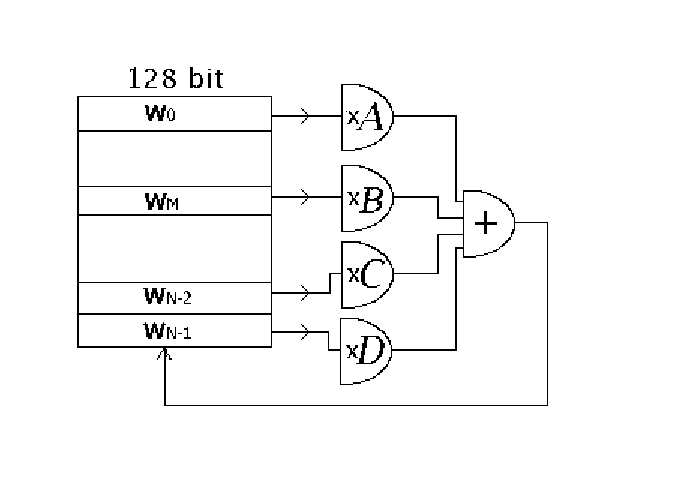
\includegraphics[width=0.7\linewidth]{sfmt-a.eps}
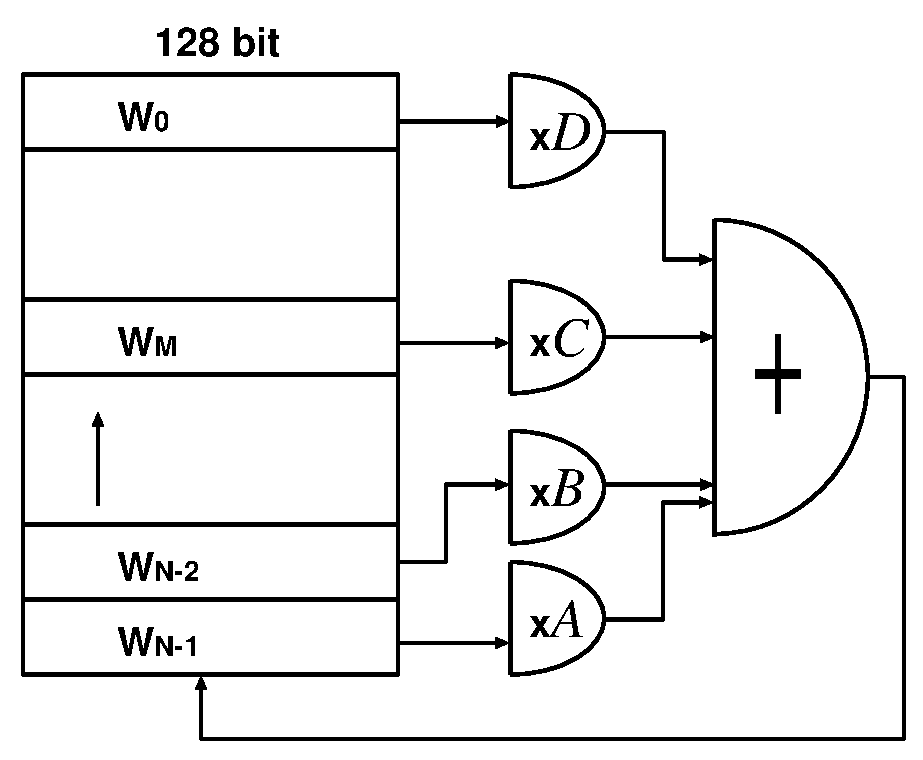
\includegraphics[width=0.7\linewidth]{sfmt-a2.eps}
\\
Figure 2: The transition function of Simple and Fast MT.

$\bw_0$ and $\bw_M$ are read from the array, but

$\bw_{N-2}$ and $\bw_{N-1}$ can be read from the registers.
\end{center}

\newpage
Reading $\bw_0$ and $\bw_M$ from the array takes some time, and 

the CPU can compute $\bw_{n-2}C$ and $\bw_{n-1}D$ in the meanwhile.

The linear transformations $A,B,C,D$ are as follows.
\begin{itemize}
\item 
%$x D := (x \stackrel{128}{>>} 8) \oplus x.$
$\bw A := (\bw \stackrel{128}{>>} 24) \oplus \bw.$
%??? different from the figure below???

This notation means that $\bw A$ is regarded
as a single 128-bit integer, and 
is shifted to the right by 24 bits.

(There is such a SIMD operation).

$\oplus$ means the exclusive-or.

\item
$\bw B := (\bw \stackrel{32}{>>} 1) \& \mbox{\tt (a constant 128-bit mask)}.$

This notation means that $\bw$ is considered to be 
a quadruple of $32$-bit integers, and
%each $32$-bit integer is shifted to the left by 20 bits.
each $32$-bit integer is shifted to the left by 1 bit,
and $\&$ means the bitwise AND. 

\newpage

\item 
$\bw C := (\bw \stackrel{128}{>>} 8).$

$(\bw \stackrel{128}{>>} 8)$ is 128-bitwise right shift as above.

\item
%$x A := (x \stackrel{32}{<<} 20).$
$\bw D := (\bw \stackrel{32}{<<} 11).$

$(\bw \stackrel{32}{<<} 11)$ is 32-bitwise right shift as above.

\end{itemize}
All these instructions are available in 
both Intel's SSE2 \\
and PowerPC's altivec SIMD instruction set.

\newpage
{\bf SIMD instructions:} 
$\stackrel{128}{<<}\quad$ and $\quad\stackrel{32}{<<}$.
\begin{center}
\includegraphics[width=0.7\linewidth]{simd-shift.eps}
\\
Figure 3: Samples of SIMD instructons.
\end{center}

\newpage
The figure below shows SFMT19937 with period $2^{19937}-1$.

There are four shift-operations, one bit-mask, and exclusive-or's.

\begin{center}
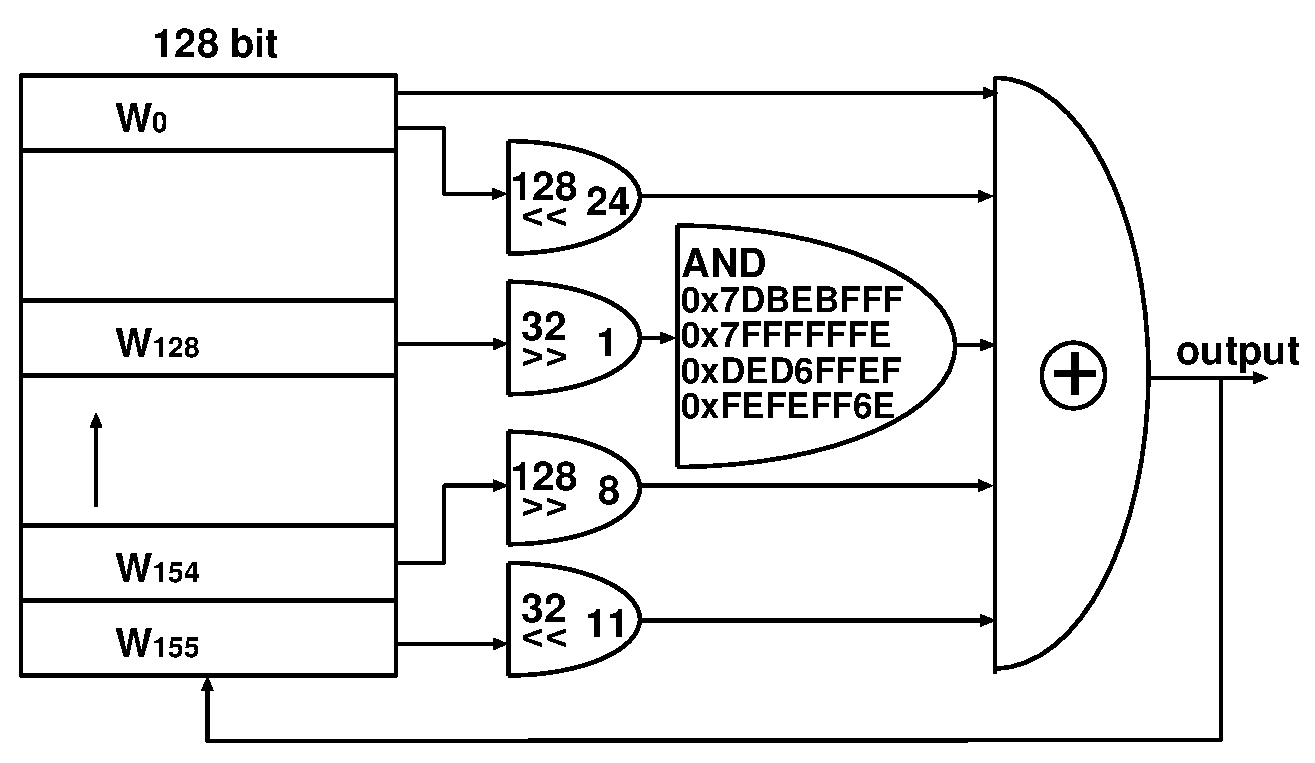
\includegraphics[width=0.7\linewidth]{sfmt-b2.eps}
\\
Figure 4: Concrete description of SFMT19937.
\end{center}

\newpage
{\bf 4. How to select these parameters.}

Write: 
\begin{itemize}
\item a code computing the (lower bound of) period

(which will be explained in Matsumoto's talk.)
\item  a code computing the dimension of equidistribution (DE).

(Here is a difficulty to treat 128-bit integer generator 

as a 32-bit integer generator,
which we omit here because of the lack of time.)
%%% 20060809
%
%later in this talk.)

\item a code measuring the speed.
\end{itemize}

\newpage
\begin{enumerate}
\item 
Decide a type of recursion by try-and-error,

using a small model (e.g. $\dim S = 607$)

(paying attentions to the speed, period, and DE).
\item
Search for the parameters 
%with period $\leq 2^{19937}-1$ 
with period $\geq 2^{19937}-1$ 

($\sim 10$ sets of parameters found per a day).
\item
Select the best parameters with respect to DE.
\end{enumerate}

\newpage
\noindent
{\bf 5. Comparison of speed}
\begin{description}
  \item Generators
    \begin{itemize}
    \item MT: Mersenne Twister with period $2^{19937}-1$ ('98).
    \item MT(SIMD): MT using SIMD instruction set.
    \item SFMT: Simple and Fast MT with period $2^{19937}-1$.
    \item SFMT(SIMD): SFMT using SIMD instruction set.
    \end{itemize}
  \item CPUs
    \begin{itemize}
      \item Pentium M 1.4GHz
      \item Pentium IV 3GHz
      \item Athlon 64 3800+
      \item Power PC G4 1.33GHz  
    \end{itemize}
    \newpage
    \item Output
      \begin{description}
      \item[block]: Generate $(634 \times 128)$ of 32-bit integers 
        in an array,
        
        616 times iterated ($\to 99999744\sim 10^8$ generations).
      \item[seq]: Generate $10^8$ of 32-bit integers sequentially,
        one by one.
      \end{description}
    \end{description}

\newpage
\begin{center}
The time (sec.) required for $10^8$ 
of 32-bit integer generations:

Pentium M 1.4GHz. 

\vskip 2mm
\begin{tabular}{|c||c|c|c|c|c|}
\hline
output & MT & MT{\Large(SIMD)} & SFMT & SFMT{\Large (SIMD)} & compiler
 \\ \hline \hline
 block   & 0.903(sec.) & \textcolor{blue}{0.479}
 & 0.584 & \textcolor{red}{0.256} &    \\ \cline{2-5}
 (ratio) & 3.53\phantom{0}  & 1.87\phantom{0}  & 2.28\phantom{0}  & 1.00\phantom{0}  & intel C/C++ \\ \cline{1-5}
 seq     & 1.112(sec.) & 1.016 & 1.007 & 0.776 & ver. 9.0\\ \cline{2-5}
 (ratio) & 1.43\phantom{0} & 1.31\phantom{0}  & 1.30\phantom{0}  & 1.00\phantom{0}  &  \\ \hline
\end{tabular}
\end{center}

\textcolor{blue}{blue} the fastest in MT

\textcolor{red}{red} the fastest in SFMT
\begin{itemize}
  \item SFMT coded in SIMD is nearly 2 (1.87) times faster than MT
 coded in SIMD.
  \item the fastest SFMT is about 3.5 times faster than original MT.
\end{itemize}
\newpage
\begin{center}
The time (sec.) required for $10^8$ 
of 32-bit integer generations:

Pentium IV 3GHz. 

\vskip 2mm
\begin{tabular}{|c||c|c|c|c|c|}
\hline
output & MT & MT{\Large(SIMD)} & SFMT & SFMT{\Large (SIMD)} & compiler
\\ \hline \hline
 block & 0.498(sec.) & \textcolor{blue}{0.300}
 & 0.387 & \textcolor{red}{0.175} & \\ \cline{2-5}
(ratio)& 2.85\phantom{0} & 1.71\phantom{0}  & 2.21\phantom{0}
  & 1.00\phantom{0}  & intel C/C++\\ \cline{1-5}
 seq   & 0.847(sec.) & 0.724 & 0.648 & 0.449 & ver. 9.0 \\\cline{2-5}
(ratio)& 1.89\phantom{0} & 1.61\phantom{0}  & 1.44\phantom{0}
  & 1.00\phantom{0}  &  \\ \hline
\end{tabular}
\end{center}
\textcolor{blue}{blue} the fastest in MT

\textcolor{red}{red} the fastest in SFMT
\begin{itemize}
  \item SFMT coded in SIMD is nearly 2 (1.71) times faster than MT
 coded in SIMD.
  \item the fastest SFMT is about 3 (2.85) times faster than original MT.
\end{itemize}

\newpage
\begin{center}
The time (sec.) required for $10^8$ 
of 32-bit integer generations:

Athlon 64 3800+ (2.4GHz)

\vskip 2mm
\begin{tabular}{|c||c|c|c|c|c|}
\hline
output & MT & MT{\Large(SIMD)} & SFMT & SFMT{\Large (SIMD)} & compiler
\\ \hline \hline
block & 0.543(sec.) & \textcolor{blue}{0.264}
 & 0.272 & \textcolor{red}{0.112} & \phantom{intel C/C++}\\
 \cline{2-5}
(ratio)& 4.85\phantom{0} & 2.36\phantom{0}  & 2.43\phantom{0} & 1.00\phantom{0} & gcc \\ \cline{1-5}
seq & 0.487(sec.) & 0.319 & 0.407 & 0.312 & ver. 4.0.2\\ \cline{2-5}
(ratio)& 1.56\phantom{0} & 1.02\phantom{0}  & 1.30\phantom{0} & 1.00\phantom{0} & \\ \hline
\end{tabular}
\end{center}
\textcolor{blue}{blue} the fastest in MT

\textcolor{red}{red} the fastest in SFMT
\begin{itemize}
  \item SFMT coded in SIMD is over 2 (2.36) times faster than MT
 coded in SIMD.
  \item the fastest SFMT is over 4 (4.35) times faster than original MT (seq).
\end{itemize}

\newpage
\begin{center}
The time (sec.) required for $10^8$ 
of 32-bit integer generations:

Power PC G4 1.33GHz

\vskip 2mm
\begin{tabular}{|c||c|c|c|c|c|}
\hline
output & MT & MT{\Large(SIMD)} & SFMT & SFMT{\Large (SIMD)} & compiler
\\ \hline \hline
block &1.406(sec.) & \textcolor{blue}{0.479}
 & 0.919 & \textcolor{red}{0.176} & \phantom{intel C/C++}\\ \cline{2-5}
(ratio)& 7.99\phantom{0} & 2.72\phantom{0}  & 5.22\phantom{0} & 1.00\phantom{0} & gcc \\ \cline{1-5}
 seq & 0.942(sec.) & 0.543 & 0.974 & 0.495 & ver.4.0.0 \\ \cline{2-5}
(ratio)& 1.90\phantom{0} & 1.10\phantom{0} & 1.97\phantom{0} & 1.00\phantom{0} & \\ \hline
\end{tabular}
\end{center}
\textcolor{blue}{blue} the fastest in MT

\textcolor{red}{red} the fastest in SFMT
\begin{itemize}
  \item SFMT coded in SIMD is nearly 3 (2.72) times faster than MT
 coded in SIMD.
  \item the fastest SFMT is over 5 (5.35) times faster than original MT (seq).
\end{itemize}

\newpage
\noindent
{\bf 6. Dimension of equidistribution} (DE).

{\bf Definition.} 
A periodic sequence with period $P$
$$\bx_0, \bx_1, \ldots, \bx_{P-1}, \bx_P=\bx_0, \ldots$$
of $v$-bit integers is said to be {\em $k$-dimensionally equidistributed}
if any $kv$-bit pattern occurs equally often as a $k$-tuple
$$
(\bx_i, \bx_{i+1}, \ldots, \bx_{i+k-1})
$$
for a period $i=0,\ldots, P-1$. 

(The all-zero pattern occurs once less often than the others.)

\newpage
A periodic sequence of 32-bit integers is said to be
{\em $k$-dimensionally equidistributed with $v$-bit accuracy}
if the most significant $v$ bits of each integer are
$k$-dimensionally equidistributed. 

We denote by $k(v)$ the maximum such $k$. 

\vskip 5mm
We have an upperbound 
$$
k(v) \leq \lfloor \log_2 (P+1) / v \rfloor, 
$$
and define the \textcolor{blue}{dimension defect} $d(v)$ at $v$
as the gap between the bound and the realized DE:
$$
d(v):= \lfloor \log_2 (P+1) / v \rfloor - k(v) \geq 0, 
$$
and the \textcolor{blue}{total dimension defect} $\Delta$
as the sum of these gaps 
$$
\Delta := \sum_{v=1}^{32}(\lfloor \log_2 (P+1) / v \rfloor -k(v)).
$$

\newpage
{\bf 7. Comparison of DE, between MT and SFMT.}
\begin{center}
\LARGE
\begin{tabular}{|c|rr||c|rr||c|rr||c|rr|} \hline
$v$ & MT & SFMT & $v$ & MT & SFMT & $v$ & MT & SFMT & $v$ & MT & SFMT\\ \hline
$d(1)$& 0 & \textcolor{red}{3}
 &$d(9)$& 346 & 1 & $d(17)$ & 549 & 543 & $d(25)$ & 174 & 173\\
$d(2)$& 0 & \textcolor{red}{1} 
&$d(10)$& 124 & 120 & $d(18)$ & 484 & 478 & $d(26)$ & 143 & 142\\
$d(3)$& 405 & 0 &$d(11)$& 564 & 0 & $d(19)$ & 426 & 420 & $d(27)$ & 115 & 114\\
$d(4)$& 0 & \textcolor{red}{1}
 &$d(12)$& 415 & 29 & $d(201)$ & 373 & 372 & $d(28)$ & 89 & 88\\
$d(5)$& 249 & 1 &$d(13)$& 287 & 270 & $d(21)$ & 326 & 325 & $d(29)$ & 64 & 63\\
$d(6)$& 207 & 1 &$d(14)$& 178 & \textcolor{red}{180}
 & $d(22)$ & 283 & 282 & $d(30)$ & 41 & 40\\
$d(7)$& 355 & 0 &$d(15)$& 83 & \textcolor{red}{85}
 & $d(23)$ & 243 & 242 & $d(31)$ & 20 & 19\\
$d(8)$& 0 & \textcolor{red}{1} &$d(16)$& 0 & \textcolor{red}{2}
 & $d(24)$ & 207 & 206 & $d(32)$ & 0 & \textcolor{red}{1} \\ \hline
\end{tabular}\\
\vskip 10mm
\begin{tabular}{crr}\hline
 & MT & SFMT \\ \hline
  $\Delta$ & 6750 & 4203 \\\hline
\end{tabular}
\end{center}
At most $v$ SFMT has better DE than MT, but at some $v$ SFMT
 has worse DE than MT
(which is colored \textcolor{red}{red}).
\newpage
\begin{center}
%\parbox{17cm}{
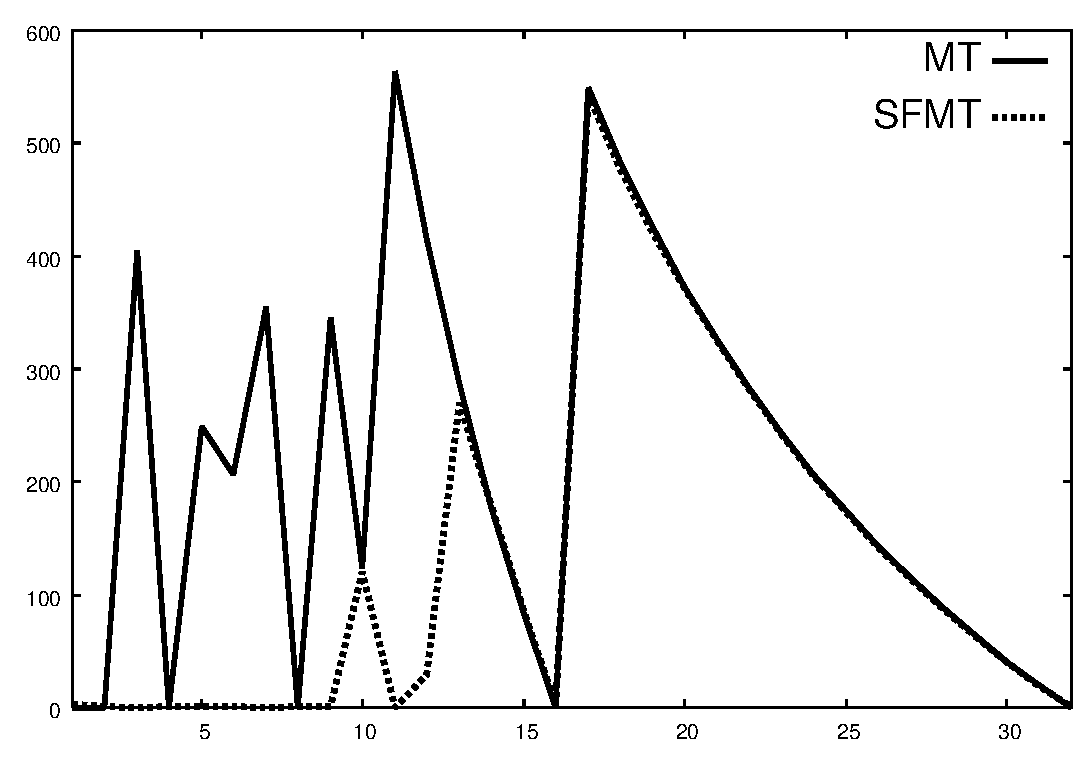
\includegraphics[width=0.8\linewidth,height=0.7\textheight,
keepaspectratio]{delta.eps}
\\
Figure 5: $d(v)$ gaps from the upperbounds.

The $x$-axis: $v=1,2,\ldots, 32$.

The $y$-axis: $d(v)$ for 
MT(\textcolor{red}{red}) and SFMT(\textcolor{green}{green}).
%}
\end{center}
%Note: WELL (Panneton-L'Ecuyer-Matsumoto) generators 
%has $\Delta = 0$, but a little slower than MT.

\newpage
{\bf 8. Conclusion.}
\begin{itemize}
\item We proposed Simple and Fast Mersenne Twister (SFMT). 
\item Almost twice faster than (SIMD-based) Mersenne Twister.
\item Better dimensions of equidistribution $k(v)$ than MT19937. 

%(at most values of $v$).
\end{itemize}
\vspace{\fill}
\begin{center}
This is the end of my talk. Thank you for listenning.
\end{center}
\vskip 1cm

\newpage
{\bf Appendix A: Computation of DE.}

Put
$$
\begin{array}{l}
I:=t^{-1}\cdot \F2[[t^{-1}]]
=\{a_{-1}t^{-1}+a_{-2}t^{-2}+\cdots \}
. \\
\end{array}
$$
Define the ultra norm on $I$ by 

$$|t^{-1}|=1/2, \quad |t^{-2}|=2^{-2}, \ldots.$$

Define the ultra norm on $I^v$ by
$$
|(b_1,\ldots,b_v)|:= \max_{i=1,2,\ldots,v} \{|b_i|\}.
$$

\newpage
Assume 
$O=\F2^v$, and 
the output sequence from $s \in S$
is 
$$
\begin{array}{c}
(\textcolor{red}{x_{11}},x_{12},\ldots,\textcolor{blue}{x_{1v}}) \in \F2^{v}\\
(\textcolor{red}{x_{21}},x_{22},\ldots,\textcolor{blue}{x_{2v}}) \in \F2^{v}\\
\vdots
\end{array}
$$
Define its generating function: 
$$
o_\infty(s):=(\sum_{i=1}^\infty \textcolor{red}{x_{i1}}t^{-i}, 
\sum_{i=1}^\infty x_{i2}t^{-i}, \ldots,
\sum_{i=1}^\infty \textcolor{blue}{x_{iv}}t^{-i}
) \in I^v.
$$

{\bf Theorem} (Couture-L'Ecuyer-Tezuka '93).
\begin{center}
The sequence has DE$\geq k$ 
$\Leftrightarrow$ 
$o_\infty(S) + t^{-k}I^v = I^v$ \\
$\Leftrightarrow$
$o_\infty(S)$ has the covering radius $\leq 2^{-k-1}$.
\end{center}

The covering radius can be computed by 
Lenstra's shortest basis algorithm (Lattice Method).

\newpage
Difficulty in SFMT: divide each 128-bit integer 
into four 32-bit integers 

$\Rightarrow$
The Lattice Method can not be used as it is.

But a minor modification solves this.

\vskip 5mm
Let $x_0, x_1, x_2, \ldots \in \F2^{128}$ be the
128-bit output sequence of SFMT.

Let us partition $x_i$ into four 32-bit integers:
$$
x_i =: (x_i[3], x_i[2], x_i[1], x_i[0]).
$$
Then the 32-bit output sequence of SFMT is
$$
\ldots, x_i[0], x_i[1], x_i[2], x_i[3], x_{i+1}[0], \cdots.
$$

\newpage
{\bf Definition.}
Let $m \in \{0,1,2,3\}$.

Let SFMT[$m$] denote the above
sequence with first $m$ words are discarded:
e.g. SFMT[1] denotes
$$
x_0[1], x_0[2], x_0[3], x_1[0], x_1[1], \ldots,
$$
and SFMT[$m$]$^v$ its $v$-bit truncations
\def\MSB{{\mbox{MSB}}}
$$
x_0[1]^v, x_0[2]^v, x_0[3]^v, x_1[0]^v, x_1[1]^v, \ldots,
$$
where $x^v$ means the $v$ most significant bits of $x$.


\vskip 3mm
{\bf Proposition.}

SFMT$^v$ has DE$ \geq k$ 
$\Leftarrow$

~~~SFMT[$m$]$^v$ has ``DE$ \geq k$''
for $m=0,1,2,3$.

Note: $\Rightarrow$ holds under a mild assumption.

\newpage
{\bf Definition.}
Concatenate every quadruples of outputs
of SFMT[$m$]$^v$, and denote it by cSFMT[$m$]$^v$.

E.g. cSFMT[1]$^v$ is a 128-bit integer sequence
$$
\begin{array}{c}
(x_0[1]^v, x_0[2]^v, x_0[3]^v, x_1[0]^v), \\
(x_1[1]^v, x_1[2]^v, x_1[3]^v, x_2[0]^v), \\
 \vdots.
\end{array}
$$

\newpage 
{\bf Theorem.} Let DE and $o_\infty$ be those of cSFMT[$m$]$^v$.

DE$\geq 4\ell$
$\Leftarrow$
$
o_\infty(S) + (t^\ell I^v,  t^\ell I^v,  t^\ell I^v, t^\ell I^v)
=I^{4v}.
$

DE$\geq 4\ell+1$
$\Leftarrow$
$
o_\infty(S) + (t^{\ell+1} I^v,  t^\ell I^v,  t^\ell I^v, t^\ell I^v)
=I^{4v}.
$

DE$\geq 4\ell+2$
$\Leftarrow$
$
o_\infty(S) + (t^{\ell+1} I^v,  t^{\ell+1} I^v,  t^\ell I^v, t^\ell I^v)
=I^{4v}.
$

DE$\geq 4\ell+3$
$\Leftarrow$
$
o_\infty(S) + (t^{\ell+1} I^v,  t^{\ell+1} I^v,  t^{\ell+1} I^v, t^\ell I^v)
=I^{4v}.
$

Note: $\Rightarrow$ holds under a mild assumption.

\newpage
The latter conditions can be computed by Lattice method
with the weighted norm: e.g., for the last case, define
$$
|(b[0], b[1], b[2], b[3])| := \max \{2|b[0]|, 2|b[1]|, 2|b[2]|, |b[3]|\}.
$$
Then the length of the shortest lattice base is $\leq 2^{-\ell-1}$

~~~$\Rightarrow$ DE$\geq 4\ell +3$. 

Note: $\Leftarrow$ holds under a mild assumption.

\vskip 1cm
\begin{center}
This is the end of my talk.
\end{center}

\newpage
{\bf Appendix B: block output}

Here is a rough sketch of {\bf block output}.

%The idea of {\bf fill\_array\_block}
\begin{center}
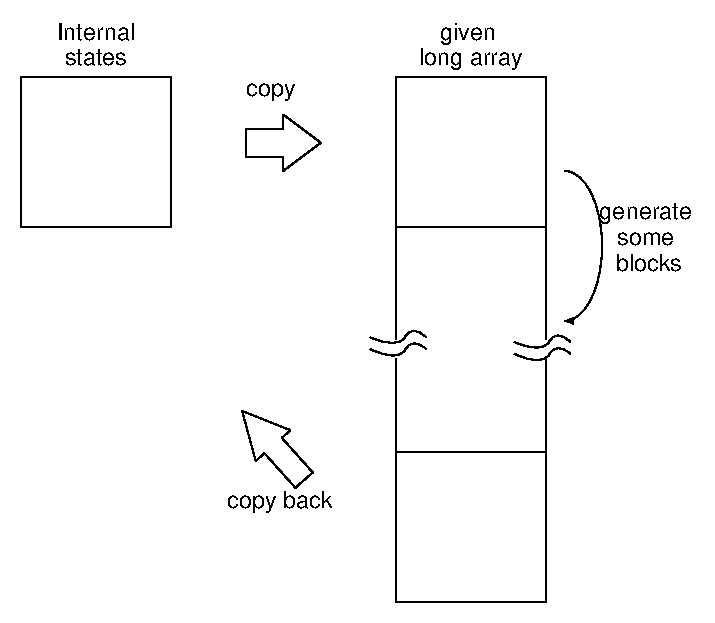
\includegraphics[width=0.7\linewidth,height=0.7\textheight,
keepaspectratio]{fill_array.eps}
\\
Figure B-1: block output
\end{center}
\newpage
And Figure B-1 is same as following steps.

Step 1. (first N - M words) \\
~~~~Read from the internal memory and write to the given array.

Step 2. (N - M + 1 to N words) \\
~~~~Read from the internal memory and given array, and 
write to the given array.

Step 3. (some multiple of 624 words + 624 - M words)\\
~~~~Read from the given array and write to the given array.

Step 4. (last N words)\\
~~~~Read from the given array and write to the given array and
 the internal memory.

Step 5. (MT only)\\
~~~~Temper the all elements of given array. 

\vskip 1cm
\begin{center}
This is the end of my talk.
\end{center}
\end{document}
\newpage
MT19937ar calculates next 624 states at once,
and output pseudo-random numbers sequencially.

\vspace{\baselineskip}
if (mti $>$= N) \{\\
~~~~calculate next 624 states.\\
\}\\
tempering...\\
output.\\

The condition part of {\bf if} statement is evaluated every time.
And jump instruction may be executed every time.

We think it's much faster when PRNG outputs
some blocks of numbers at once.

\newpage
{\bf 7-3} Calculate 32-bit $k(v)$ of 128-bit recursion formula PRMG

\begin{center}
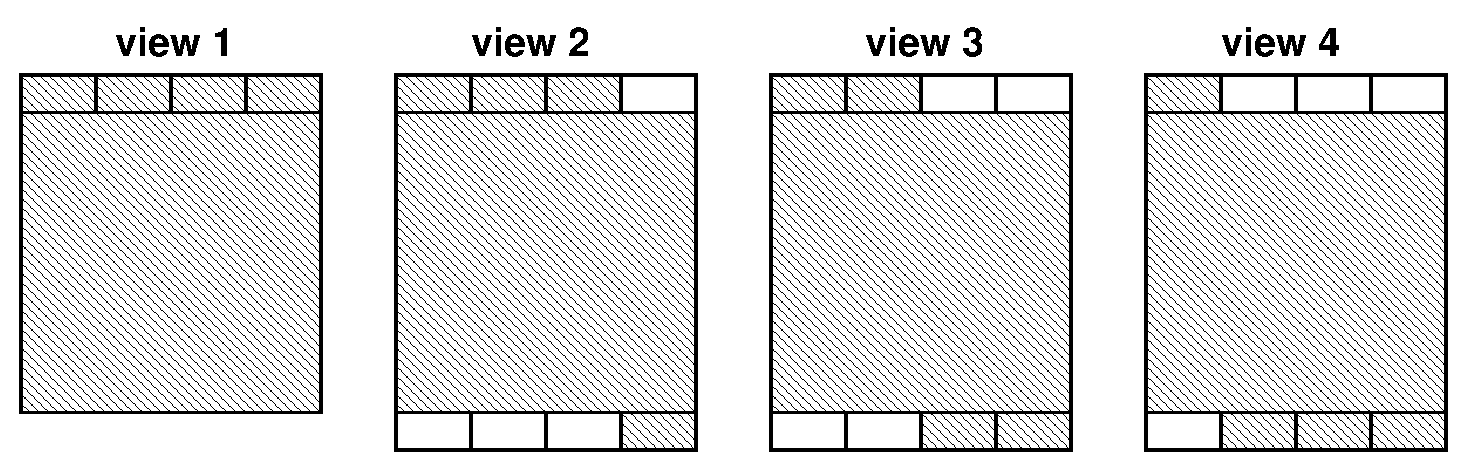
\includegraphics[width=\linewidth,height=0.6\textheight,
keepaspectratio]{view.eps}
\\
Figure 6: get minimum $k$-distributio of four views
\end{center}
\newpage

\begin{center}
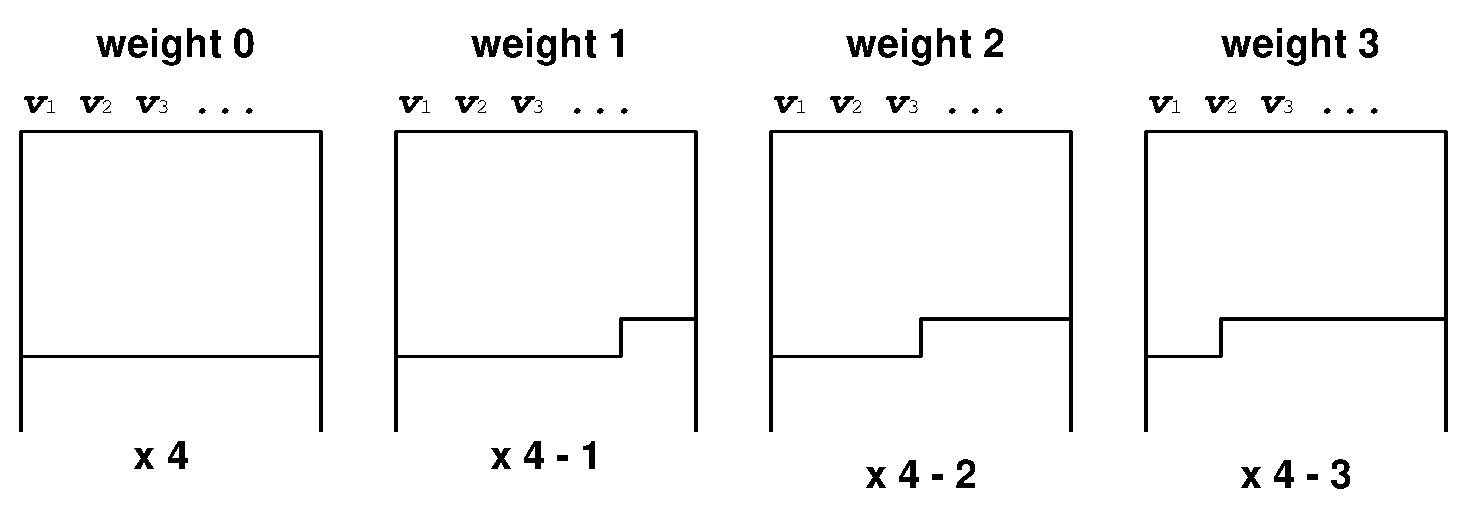
\includegraphics[width=\linewidth,height=0.6\textheight,
keepaspectratio]{weight.eps}
\\
Figure 7: weighted norm
\end{center}


\newpage
\noindent
{\bf 9 Concluding Remarks}

We conclude that SFMT is fast version of Mersenne Twister.

\newpage
Endian\\
When use 32-bit and 128-bit integers together,

\begin{center}
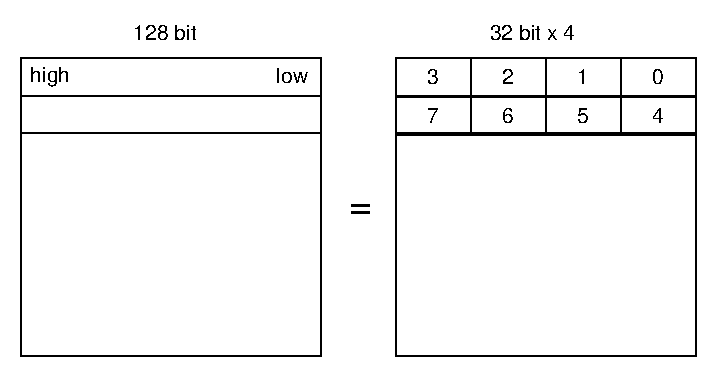
\includegraphics[width=0.7\linewidth]{little-endian.eps}
\\
Figure 5: Little Endian
\end{center}
\newpage
\noindent
{\bf 7 Simple and Fast MT (SFMT)}

Now one word is 128-bit width,
and we read $\bw_{N-1}$ and $\bw_{N-2}$.

\begin{center}
%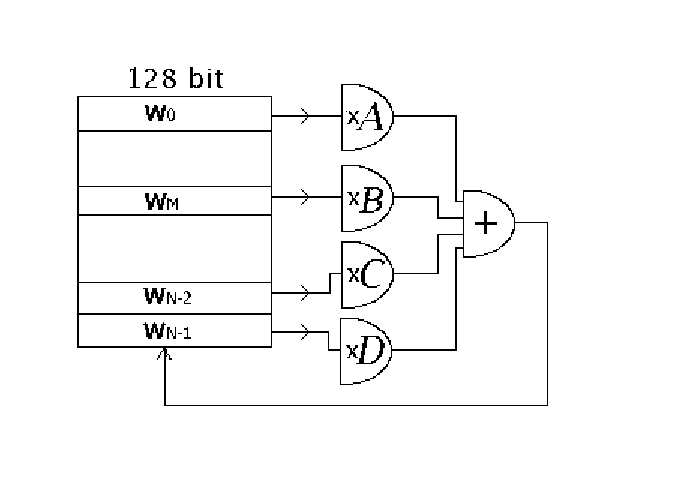
\includegraphics[width=0.7\linewidth]{sfmt-a.eps}
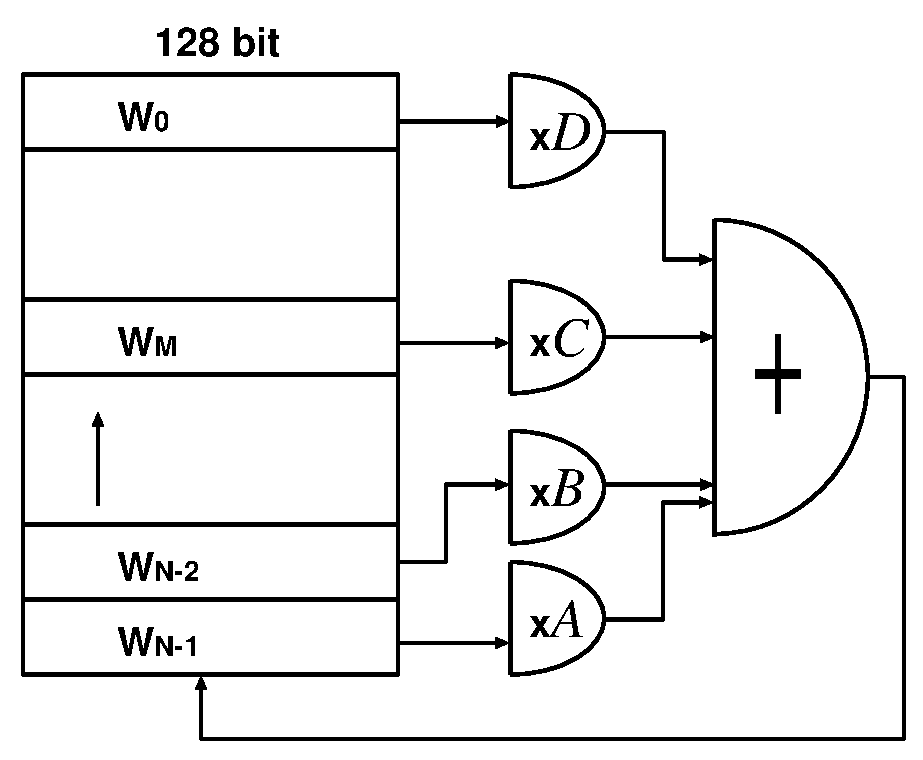
\includegraphics[width=0.7\linewidth]{sfmt-a2.eps}
\\
Figure 6: The transition function of Simple and Fast MT
\end{center}
SFMT is currently implemented for Intel's SSE2 and PowerPC's altivec SIMD
instruction set.



\end{document}




